% LaTeX path to the root directory of the current project, from the directory in which this file resides
% and path to econtexPaths which defines the rest of the paths like \FigDir
\providecommand{\econtexRoot}{}\renewcommand{\econtexRoot}{.}
\providecommand{\econtexPaths}{}\renewcommand{\econtexPaths}{\econtexRoot/Resources/econtexPaths}
% The \commands below are required to allow sharing of the same base code via Github between TeXLive on a local machine and Overleaf (which is a proxy for "a standard distribution of LaTeX").  This is an ugly solution to the requirement that custom LaTeX packages be accessible, and that Overleaf seems to ignore symbolic links (even if they are relative links to valid locations)
\providecommand{\econtex}{\econtexRoot/Resources/texmf-local/tex/latex/econtex}
\providecommand{\econtexSetup}{\econtexRoot/Resources/texmf-local/tex/latex/econtexSetup}
\providecommand{\econtexShortcuts}{\econtexRoot/Resources/texmf-local/tex/latex/econtexShortcuts}
\providecommand{\econtexBibMake}{\econtexRoot/Resources/texmf-local/tex/latex/econtexBibMake}
\providecommand{\econtexBibStyle}{\econtexRoot/Resources/texmf-local/bibtex/bst/econtex}
\providecommand{\econtexBib}{economics}
\providecommand{\notes}{\econtexRoot/Resources/texmf-local/tex/latex/handout}
\providecommand{\handoutSetup}{\econtexRoot/Resources/texmf-local/tex/latex/handoutSetup}
\providecommand{\handoutShortcuts}{\econtexRoot/Resources/texmf-local/tex/latex/handoutShortcuts}
\providecommand{\handoutBibMake}{\econtexRoot/Resources/texmf-local/tex/latex/handoutBibMake}
\providecommand{\handoutBibStyle}{\econtexRoot/Resources/texmf-local/bibtex/bst/handout}

\providecommand{\FigDir}{\econtexRoot/Figures}
\providecommand{\CodeDir}{\econtexRoot/Code}
\providecommand{\DataDir}{\econtexRoot/Data}
\providecommand{\SlideDir}{\econtexRoot/Slides}
\providecommand{\TableDir}{\econtexRoot/Tables}
\providecommand{\ApndxDir}{\econtexRoot/Appendices}

\providecommand{\ResourcesDir}{\econtexRoot/Resources}
\ifnum\pdfshellescape=1
\providecommand{\rootFromOut}{..} % Path back to root directory from output-directory
\providecommand{\LaTeXGenerated}{\econtexRoot/LaTeX} % Put generated files in subdirectory
\providecommand{\EqDir}{\econtexRoot/Equations} % Put generated files in subdirectory
\else
\providecommand{\rootFromOut}{.} % Path back to root directory 
\providecommand{\LaTeXGenerated}{\econtexRoot/} % Put generated files in main directory (because not allowed in subdirectory)
\providecommand{\EqDir}{\econtexRoot/} % Put generated files in main directory
\fi
\providecommand{\econtexPaths}{\econtexRoot/Resources/econtexPaths}
\providecommand{\LaTeXInputs}{\econtexRoot/Resources/LaTeXInputs}

\documentclass[\econtexRoot/BufferStockTheory]{subfiles}
% LaTeX path to the root directory of the current project, from the directory in which this file resides
% and path to econtexPaths which defines the rest of the paths like \FigDir
\providecommand{\econtexRoot}{}\renewcommand{\econtexRoot}{.}
\providecommand{\econtexPaths}{}\renewcommand{\econtexPaths}{\econtexRoot/Resources/econtexPaths}
% The \commands below are required to allow sharing of the same base code via Github between TeXLive on a local machine and Overleaf (which is a proxy for "a standard distribution of LaTeX").  This is an ugly solution to the requirement that custom LaTeX packages be accessible, and that Overleaf seems to ignore symbolic links (even if they are relative links to valid locations)
\providecommand{\econtex}{\econtexRoot/Resources/texmf-local/tex/latex/econtex}
\providecommand{\econtexSetup}{\econtexRoot/Resources/texmf-local/tex/latex/econtexSetup}
\providecommand{\econtexShortcuts}{\econtexRoot/Resources/texmf-local/tex/latex/econtexShortcuts}
\providecommand{\econtexBibMake}{\econtexRoot/Resources/texmf-local/tex/latex/econtexBibMake}
\providecommand{\econtexBibStyle}{\econtexRoot/Resources/texmf-local/bibtex/bst/econtex}
\providecommand{\econtexBib}{economics}
\providecommand{\notes}{\econtexRoot/Resources/texmf-local/tex/latex/handout}
\providecommand{\handoutSetup}{\econtexRoot/Resources/texmf-local/tex/latex/handoutSetup}
\providecommand{\handoutShortcuts}{\econtexRoot/Resources/texmf-local/tex/latex/handoutShortcuts}
\providecommand{\handoutBibMake}{\econtexRoot/Resources/texmf-local/tex/latex/handoutBibMake}
\providecommand{\handoutBibStyle}{\econtexRoot/Resources/texmf-local/bibtex/bst/handout}

\providecommand{\FigDir}{\econtexRoot/Figures}
\providecommand{\CodeDir}{\econtexRoot/Code}
\providecommand{\DataDir}{\econtexRoot/Data}
\providecommand{\SlideDir}{\econtexRoot/Slides}
\providecommand{\TableDir}{\econtexRoot/Tables}
\providecommand{\ApndxDir}{\econtexRoot/Appendices}

\providecommand{\ResourcesDir}{\econtexRoot/Resources}
\ifnum\pdfshellescape=1
\providecommand{\rootFromOut}{..} % Path back to root directory from output-directory
\providecommand{\LaTeXGenerated}{\econtexRoot/LaTeX} % Put generated files in subdirectory
\providecommand{\EqDir}{\econtexRoot/Equations} % Put generated files in subdirectory
\else
\providecommand{\rootFromOut}{.} % Path back to root directory 
\providecommand{\LaTeXGenerated}{\econtexRoot/} % Put generated files in main directory (because not allowed in subdirectory)
\providecommand{\EqDir}{\econtexRoot/} % Put generated files in main directory
\fi
\providecommand{\econtexPaths}{\econtexRoot/Resources/econtexPaths}
\providecommand{\LaTeXInputs}{\econtexRoot/Resources/LaTeXInputs}

\onlyinsubfile{% https://tex.stackexchange.com/questions/463699/proper-reference-numbers-with-subfiles
    \csname @ifpackageloaded\endcsname{xr-hyper}{%
      \externaldocument{\econtexRoot/BufferStockTheory}% xr-hyper in use; optional argument for url of main.pdf for hyperlinks
    }{%
      \externaldocument{\econtexRoot/BufferStockTheory}% xr in use
    }%
    \renewcommand\labelprefix{}%
    % Initialize the counters via the labels belonging to the main document:
    \setcounter{equation}{\numexpr\getrefnumber{\labelprefix eq:Dummy}\relax}% eq:Dummy is the last number used for an equation in the main text; start counting up from there
}


\onlyinsubfile{\externaldocument{BufferStockTheory}}

\begin{document}\label{sec:ApndxConditionDiagrams}
\hypertarget{ApndxConditionDiagrams}{}
\section{Relational Diagrams for the Inequality Conditions}

\subsection{For the Unconstrained Perfect Foresight Model}

\providecommand{\figName}{InequalityPFGICFHWCRIC}
\providecommand{\figFile}{\figName}
\hypertarget{\figFile}{}
\hypertarget{\figName}{}
\begin{figure}[h]
  \centerline{
    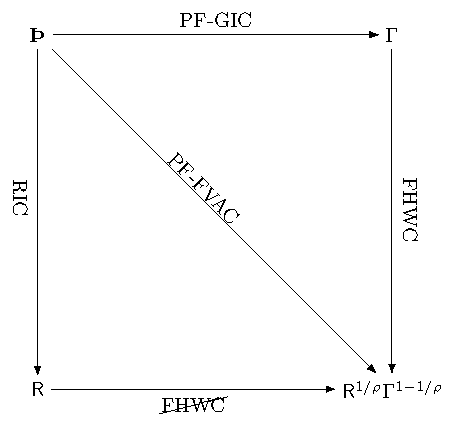
\includegraphics[width=3in]{\FigDir/RelatePFGICFHWCRICPFFVAC}
  }
  \caption{Relation of \PFGIC, \FHWC, \RIC, and \PFFVAC} \label{fig:RelatePFGICFHWCRICPFFVAC}
  \footnotesize{Arrows reflect the direction of the relationship; an arrowhead points to the larger of the two quantities being compared.  For example, the topmost arrow, pointing from $\Pat$ to $\PGro$ indicates that $\PGro > \Pat$.}
\end{figure}

% %\begin{verbatimwrite}{\figName}
% \hypertarget{InequalityPFGICFHWCRIC}{}

% \tikzset{node distance=6cm, auto, >=latex}
% \begin{figure}[h]
%   \label{fig:InequalityPFGICFHWCRIC}
%   \centerline{
%       \begin{tikzpicture}
%         \node (thorn) {$\Pat$}; % ((\Rfree \DiscFac)^{1/\CRRA} \equiv )~~
\node (gamma) [right of = thorn] {$\PGro$};
\node (thorndef) [left of = thorn,xshift=4.8cm] {$((\Rfree \DiscFac)^{1/\CRRA} \equiv)$};
\node (rfree) [below of = thorn, xshift = 2.8cm, yshift = 2cm]{${\Rfree}$};
\node (ineq)  [below of = thorn, xshift = 2.8cm, yshift = 4.5cm]{$\neq$};
%\node (strix) [left of = gamma, xshift = 4.35cm, yshift = -0.6cm] {};
%\node (striy) [left of = gamma, xshift = 2.78cm, yshift = -0.9cm] {};
%\draw[-] (strix) to (striy); 
\draw[->] (thorn) to node{\PFGIC $(\equiv \Pat < \PGro)$} (gamma);
%\draw[->] (gamma) to [out = 200, in=-10] node[below]{\PFGIC} (thorn); %\st{\textrm{PF-GIC};
\draw[->] (thorn) to node [swap] {$(\Pat < \Rfree \equiv)~~\mathrm{\RIC}$} (rfree);
\draw[->] (gamma) to node {$\mathrm{\FHWC}~~(\equiv \PGro < \Rfree) $} (rfree);

%       \end{tikzpicture}
%   }
%   \caption{Relation of {\RIC}, {\PFGIC}, and {\FHWC} in Perfect Foresight Model}
%   \footnotesize{Arrows reflect the direction of the relationship; an arrowhead points to the larger of the two quantities being compared.  For example, the topmost arrow, pointing from $\Pat$ to $\PGro$, indicates that $\PGro > \Pat$.}
% \end{figure}
% %\end{verbatimwrite}
% %\input{\FigDir/\figName}


Figure~\ref{fig:InequalityPFGICFHWCRIC} should be read as follows.  The three nodes represent the values of the absolute patience factor \Thorn, the growth factor for permanent income $\PGro$, and the riskfree interest factor $\Rfree$.  The arrows between these quantities represent imposition of the labeled condition.  For example, the uppermost arrow, pointing from {$\Pat$} to $\PGro$, reflects imposition of the {\PFGIC} condition.  To make interpretation of the diagram easy, the mathematical representation of the condition is expressed in parentheses as being equivalent ($\equiv$) to the condition.

The imposition of the negation of the $\PFGIC$ (the lower curved arrow pointing from $\PGro$ to {$\Pat$}, labeled \cncl{\PFGIC}) could have been left out, under the convention that the negation of an arrow pointing in one direction is an arrow pointing in the opposite direction.  So, for example, the negation of the {\RIC} is $\cncl{\RIC} \equiv \Pat > \Rfree$ but could be represented by moving the arrowhead from the bottom right to the top left of the line segment connecting {$\Pat$} and $\Rfree$.

Because they reflect inequalities, the implications of the arrows accumulate as the diagram is traversed.  For example, if we were to start at $\Rfree$ and then impose $\cncl{\FHWC}$, that would reverse the arrow connecting $\Rfree$ and $\PGro$.  If we were then to impose $\cncl{\PFGIC}$, we would follow the arrow to {$\Pat$}.  But  
\begin{equation}\begin{gathered}\begin{aligned}
  \cncl{\FHWC}:~~~~  \Rfree & < \PGro \notag  
  \\ \cncl{\PFGIC}:~~~~ \PGro & < \Pat %~\left(\equiv (\Rfree \DiscFac)^{1/\CRRA}\right)
                                \label{eq:cnclRIC}
  \\ \Rightarrow \cncl{\RIC}:~~~~\Rfree & < \Pat \notag,
\end{aligned}\end{gathered}\end{equation}
which illustrates another aspect of the diagram: If all arrows are reversed in a partial traversal of the diagram leading to a final step, then the arrow for the final step must also be reversed.  In this case, since both conditions leading to $\Rfree$ have had their arrows reversed, the arrow coming out of $\Rfree$ should also be reversed, implying the negation of the {\RIC} -- as \eqref{eq:cnclRIC} proved.

For clarity, further diagrams will omit multiple arrows indicating reversal of causality (in Figure~\ref{fig:InequalityPFGICFHWCRIC} there would, for example, be only a single arrow, from {$\Pat$} to $\PGro$, at the top level of the diagram).  And definitions of conditions will also be omitted henceforth.

Under these conventions, we can extend the diagram to incorporate the $\PFFVAC$ (see Figure~\ref{fig:RelatePFGICFHWCRICPFFVAC}).\footnote{For readers familiar with the \href{https://en.wikipedia.org/wiki/Commutative_diagram}{commutative diagrams}, it should be noted that this diagram is NOT commutative, because the three ways of arriving at the conclusion embodied in the diagonal arrow (the {\PFFVAC}) are NOT identical in their other implications.}

\renewcommand{\figName}{RelatePFGICFHWCRICPFFVAC}
  \begin{figure}[h]
  \hypertarget{\figName}{}
    \centerline{
      \begin{tikzpicture}
        ;;; -*- coding: utf-8; -*-
      \node (pffvafNEQpfgicPfhwc) [xshift=4cm,yshift=-1.5cm]{$\neq$};
      \node (pffvafNEQricPcancelfhwc) [xshift=1.5cm,yshift=-3.8cm]{$\neq$};
      \node (thorn) {$\Pat$};
      \node (gamma) [right of = thorn] {$\PGro$};
      \node (rfree) [below of = thorn]{$\mathsf{\Rfree}$};
%      \node (pffvacFac) [right of = rfree] {$\underbrace{\Rfree^{1/\CRRA}\PGro^{1 - 1/\CRRA}}_{\equiv \PGro} $}; % \left(\equiv (\Rfree \PGro)^{1/\CRRA}\PGro\right)
      \node (pffvacFac) [right of = rfree] {$\Rfree^{1/\CRRA}\PGro^{1 - 1/\CRRA}$}; % \left(\equiv (\Rfree \PGro)^{1/\CRRA}\PGro\right)
      \draw[->] (thorn) to node {${\PFGIC}$} (gamma);
      \draw[->] (thorn) to node [swap] [rotate=-90,yshift=-0.3cm,xshift=+0.2cm]{${\RIC}$} (rfree);
      \draw[->] (thorn) to node [swap] [rotate=-45,xshift=0.5cm,yshift=+0.4cm] {$\PFFVAC$} (pffvacFac);
      \draw[->] (gamma) to node [rotate=-90,xshift=-0.7cm,yshift=+0.3cm]{${\FHWC}$} (pffvacFac);
      \draw[<-] (pffvacFac) to node{\cncl{\FHWC}} (rfree); 

      \end{tikzpicture}
    }
    \caption{Relation of \PFGIC, \FHWC, \RIC, and \PFFVAC} \label{fig:RelatePFGICFHWCRICPFFVAC}
    \footnotesize{Arrows reflect the direction of the relationship; an arrowhead points to the larger of the two quantities being compared.  For example, the topmost arrow, pointing from $\Pat$ to $\PGro$ indicates that $\PGro > \Pat$.}
  \end{figure}

This diagram can be interpreted, for example, as saying  that it is possible to derive the $\PFFVAC$\footnote{in the form $\Pat < (\Rfree/\PGro)^{1/\CRRA}\PGro$} by imposing both the {\PFGIC} and the {\FHWC}; or by imposing {\RIC} and \cncl{\FHWC}.  Or, starting at the $\PGro$ node, we can follow the imposition of the {\FHWC} (twice) and then $\cncl{\RIC}$ to reach the conclusion that $\Pat < (\Rfree \PGro)^{1/\CRRA} \PGro$.  Algebraically,
\begin{equation}\begin{gathered}\begin{aligned}
  {\FHWC}:~~~ \PGro & < \Rfree \notag
  \\ \cncl{\RIC}:~~~ \Rfree & < \Pat \notag
  \\ \PGro & < \Pat \label{eq:cnclPFGIC}
\end{aligned}\end{gathered}\end{equation}
which leads to the negation of the two conditions leading into $\Pat$: \cncl{\PFGIC} is obtained directly by dividing both sides of \eqref{eq:cnclPFGIC} and \cncl{\PFFVAC} follows if we start by multipling the Return Patience Factor ({\RPF}=$\Pat/\Rfree$) by the \FHWF (=$\PGro/\Rfree$) raised to the power $1/\CRRA-1$, which is negative since we imposed $\CRRA > 1$.  {\FHWC} implies {\FHWF} $< 1$ so when {\FHWF} is raised to a negative power the result is greater than one.
Multiplying the \RPF (which exceeds 1 because \cncl{\RIC}) by a number greater than one yields a product that must be greater than one:
\begin{equation}\begin{gathered}\begin{aligned}
  1  & < \overbrace{\left(\frac{(\Rfree \DiscFac)^{1/\CRRA}}{\Rfree}\right)}^{>1 \text{~from~}\cncl{\RIC}}\overbrace{\left(\PGro/\Rfree\right)^{1/\CRRA-1}}^{\phantom{...}>1~\text{~from~} \FHWC} \notag
  \\ 1  & < \left(\frac{(\Rfree \DiscFac)^{1/\CRRA}}{(\Rfree/\PGro)^{1/\CRRA}\Rfree\PGro/\Rfree}\right) \label{eq:cnclFHWFAndcnclRICImplycnclPFFVAC}
  \\ \Rfree^{1/\CRRA}\PGro^{1 - 1/\CRRA} = (\Rfree/\PGro)^{1/\CRRA} \PGro  & < \Pat \notag
\end{aligned}\end{gathered}\end{equation}
which is one way of writing $\cncl{\PFFVAC}$.

After the warmup of constructing these conditions for the perfect foresight case, we can represent the relationships between all the conditions in both the perfect foresight case and the case with uncertainty as shown in Figure~\ref{fig:Inequalities}.

\end{document}

%\begin{verbatimwrite}{\figName}
  \tikzset{node distance=5cm, auto, >=latex}
  \begin{figure}[h]
  \hypertarget{\figName}{}
    \centerline{
      \begin{tikzpicture}
        ;;; -*- coding: utf-8; -*-
      \node (pffvafNEQpfgicPfhwc) [xshift=4cm,yshift=-1.5cm]{$\neq$};
      \node (pffvafNEQricPcancelfhwc) [xshift=1.5cm,yshift=-3.8cm]{$\neq$};
      \node (thorn) {$\Pat$};
      \node (gamma) [right of = thorn] {$\PGro$};
      \node (rfree) [below of = thorn]{$\mathsf{\Rfree}$};
%      \node (pffvacFac) [right of = rfree] {$\underbrace{\Rfree^{1/\CRRA}\PGro^{1 - 1/\CRRA}}_{\equiv \PGro} $}; % \left(\equiv (\Rfree \PGro)^{1/\CRRA}\PGro\right)
      \node (pffvacFac) [right of = rfree] {$\Rfree^{1/\CRRA}\PGro^{1 - 1/\CRRA}$}; % \left(\equiv (\Rfree \PGro)^{1/\CRRA}\PGro\right)
      \draw[->] (thorn) to node {${\PFGIC}$} (gamma);
      \draw[->] (thorn) to node [swap] [rotate=-90,yshift=-0.3cm,xshift=+0.2cm]{${\RIC}$} (rfree);
      \draw[->] (thorn) to node [swap] [rotate=-45,xshift=0.5cm,yshift=+0.4cm] {$\PFFVAC$} (pffvacFac);
      \draw[->] (gamma) to node [rotate=-90,xshift=-0.7cm,yshift=+0.3cm]{${\FHWC}$} (pffvacFac);
      \draw[<-] (pffvacFac) to node{\cncl{\FHWC}} (rfree); 

      \end{tikzpicture}
    }
    \caption{Relation of \PFGIC, \FHWC, \RIC, and \PFFVAC} \label{fig:RelatePFGICFHWCRICPFFVAC}
    \footnotesize{Arrows reflect the direction of the relationship; an arrowhead points to the larger of the two quantities being compared.  For example, the topmost arrow, pointing from $\Pat$ to $\PGro$ indicates that $\PGro > \Pat$.}
  \end{figure}
%\end{verbatimwrite}
%\input{\FigDir/\figName}


\renewcommand{\figName}{Inequalities}
%\begin{verbatimwrite}{\figName}
  \tikzset{node distance=5cm, auto, >=latex}
  \begin{figure}[h]
    \hypertarget{Inequalities}{}
    \centerline{
      \begin{tikzpicture}
                \node (thorn) {$\Pat$};
        \node (gamma) [right of = thorn, xshift = 5cm] {$\PGro$};
        \node (rfree) [below of = thorn]{$\mathsf{\Rfree}$};
        \node (pffvacFac) [right of = rfree] 
        {$\mathsf{\Rfree}^{1/\CRRA}\PGro^{1 - 1/\CRRA}$};
        \node (pThorn) [left of = thorn] {$\pZero^{1/\rho}\Pat$};
        \node (compgamma) [above of = gamma, xshift = -5cm, yshift = -2.5cm]{$\PGroAdj$};
        \node (fvacFac) [right of = thorn, yshift = -2cm]{$\mathsf{\Rfree}^{1/\CRRA}\PGrouAdj^{1 - 1/\CRRA}$};
        \draw[->] (thorn) to node {${\PFGIC}$} (gamma);
        \draw[->] (thorn) to node [swap] {${\RIC}$} (rfree);
        \draw[->] (thorn) to node [swap] {${\PFFVAC}$} (pffvacFac);
        \draw[->] (gamma) to node {${\FHWC}$} (pffvacFac);
        \draw[->] (pffvacFac) to node {${\FHWC}$} (rfree);
        \draw[->] (pThorn) to node [above]{because $\wp < 1$} (thorn);
        \draw[->] (pThorn) to node [swap] {${\WRIC}$} (rfree);
        \draw[->] (compgamma) to node [rotate=-35,xshift=-2.2cm,yshift=+0.05cm]{because $\underline{\psi} < 1$ and $\uline{\PGro} \equiv \underline{\psi} \PGro$} (gamma);
        \draw[->] (thorn) to node {${\GIC}$} (compgamma);
        \draw[->] (fvacFac) to node {} (pffvacFac);
        \draw[->] (thorn) to node {${\FVAC}$} (fvacFac);

      \end{tikzpicture}	
    }
    \caption{Relation of All Inequality Conditions} \label{fig:Inequalities}
  \end{figure}
%\end{verbatimwrite}
%\input{\FigDir/\figName}

% \onlyinsubfile{\bibliography{BufferStockTheory,economics}}


\end{document}

% Local Variables:
% eval: (setq TeX-command-list  (assq-delete-all (car (assoc "BibTeX" TeX-command-list)) TeX-command-list))
% eval: (setq TeX-command-list  (assq-delete-all (car (assoc "BibTeX" TeX-command-list)) TeX-command-list))
% eval: (setq TeX-command-list  (assq-delete-all (car (assoc "BibTeX" TeX-command-list)) TeX-command-list))
% eval: (setq TeX-command-list  (assq-delete-all (car (assoc "BibTeX" TeX-command-list)) TeX-command-list))
% eval: (setq TeX-command-list  (assq-delete-all (car (assoc "Biber"  TeX-command-list)) TeX-command-list))
% eval: (add-to-list 'TeX-command-list '("BibTeX" "bibtex ../LaTeX/%s" TeX-run-BibTeX nil t                                                                              :help "Run BibTeX") t)
% eval: (add-to-list 'TeX-command-list '("BibTeX" "bibtex ../LaTeX/%s" TeX-run-BibTeX nil (plain-tex-mode latex-mode doctex-mode ams-tex-mode texinfo-mode context-mode) :help "Run BibTeX") t)
% TeX-PDF-mode: t
% TeX-file-line-error: t
% TeX-debug-warnings: t
% LaTeX-command-style: (("" "%(PDF)%(latex) %(file-line-error) %(extraopts) -output-directory=../LaTeX %S%(PDFout)"))
% TeX-source-correlate-mode: t
% TeX-parse-self: t
% eval: (cond ((string-equal system-type "darwin") (progn (setq TeX-view-program-list '(("Skim" "/Applications/Skim.app/Contents/SharedSupport/displayline -b %n ../LaTeX/%o %b"))))))
% TeX-parse-all-errors: t
% End:
